\documentclass[10pt, a4paper,twocolumn]{article}
\usepackage[T1,T2A]{fontenc}
\usepackage[utf8]{inputenc}
\usepackage[russian, english]{babel}
% \renewcommand{\rmdefault}{cmss}
% \renewcommand{\ttdefault}{cmss}
\usepackage{amsfonts}
\usepackage{graphicx}
\graphicspath{ {images/} }
\usepackage[left=15mm, top=20mm, right=15mm, bottom=20mm]{geometry}

\title{конспект гранде}

\begin{document}
\maketitle

\begin{abstract}
Это всего лишь неловкие попытки совместить приятное с полезным - освоить большую часть матмематических команд и фукнций \LaTeX а и заодно повторить (ну или выучить) материал к коллоку. Если вам эта штукенция попалась в руки - не обращайте внимания, проходите мимо и не осуждайте неточности и грубость изложения
\end{abstract}
\tableofcontents

\section{Число сочетаний, свойства. Бином Ньютона. Примеры.}
\textsl{Презентация по теме: 03.09.24, гл. 1, пар. 1}
\\ \\
Сразу - тут могло бы быть определение факториала, но его нет в вопросе, потому нет так нет. Но для общего развития: \textsl{факториал} - это та штучка с восклицательным знаком около числа; обозначает последовательное перемножение всех чисел от 1 до данного числа. Типа, факториал числа 5 (5!) это перемножение всех чисел от 1 до пяти: $1 * 2 * 3 * 4 * 5 = 120.$ 
\\ \\
\textbf{Числом сочетаний} из n по k называется число равное $\frac{n!}{k!(n-k)!}$, при $n \leq k$. Оно обозначается как $C^{k}_n$. \\ Так же является числом неупорядоченных из k элементов множества, состоящего из n элементов. (Есть мешок из 5 яблок, мы в абсолютно случайном порядке хотим вытащить 3 яблока - $C^{3}_5 = \frac{5!}{3!(5 - 3)!}$), это так называемый \textsl{комбинаторный смысл} числа сочетаний.
\subsection{Свойства числа сочетаний}
\begin{enumerate}
\item $C^{k}_n = C^{n - k}_n$
\item $C^{0}_n = C^{n}_n = 1$
\item $C^{1}_n = C^{n - 1}_n = n$
\item $C^{k - 1}_n + C^{k}_n = C^{k}_{n+1}$ 
\end{enumerate}
В основном, чаще всего мы вспоминаем про первое и третье - особенно полезно помнить при раскрытиях биномов Ньютона, так как они обьясняют симметричность коэффициентов; про второе никто не вспоминает, но всеми ими пользуются (те самые единицы в треугольнике Паскаля как раз появляются из-за них), но да ладно. \\ \textsl{Вопроса на докозательство этих штук нет!} Чему я безусловно рада, но доказываются они буквально через раскрытие всех выражений через формулу, а дальше простая арифметика. Потому не теряемся если спросит!
\subsection{Бином Ньютона}
А, кстати, о нем.
$$(a + b)^n = a^n + C^{1}_{n} a^{n - 1} b + C^{2}_{n} a^{n - 2} b^{2} + {...} +C^{n - 1}_{n} a b^{n - 1} + b^{n}$$
Или же!
$$(a + b)^n = \displaystyle\sum_{k = 0}^{n} C^{k}_{n} a^{n - k} b^{k}$$
Тут добавить более нечего, на деле. Это буквально все по теме, что было включено в презентацию, помимо примеров, до которых вы и сами додумаетесь если вспомните квадраты или кубы сумм или разностей.

\section{Принцип математической индукции, примеры. Неравенство Бернулли.}
\textsl{Презентация по теме: 05.09.24, гл. 1, пар. 2}
\\ \\
\textbf{Принцип математической индукции}: пусть $\rho_n, n \leq 1$ - последовательность утверждений. Если 
\begin{enumerate}
\item Утверждение  $\rho_1$ верное
\item Из того, что $\rho_n$ верно, следует, что $\rho_{n + 1}$ верно. Тогда утверждение $\rho_n$ верно при всех $n \leq 1$
\end{enumerate}
Предположение о том, что $\rho_n$ верно (первая часть второго пункта) называют \textsl{индукционным предположением}. Переход от истинности $\rho_n$ к истинности $\rho_{n + 1}$ (сам второй пункт полностью) - \textsl{индукционным переходом}. Вся логика мат. индукции строится на том, что любое множество, состоящее из натуральных чисел, имеет наименьший элемент (собственно, потому она начинается с первого элемента и проверки истинности выражения на единице).
\subsection{Неравенство Бернулли}
$$(1 + x)^{n} \leq 1 + nx, x \leq -1 text{для всех} n \leq 1$$
А теперь, самое веселое, доказательство:
\begin{enumerate}
\item Проверим истинность выражения для $n = 1$:
$$(1 + x)^{1} \leq 1 + 1 * x \Leftrightarrow 1 + x \leq 1 + x$$
\item Если оно верно для $n = 1$, предположим что оно верно для $n$, тогда докажем его верность для $n + 1$
$$(x + 1)^{n + 1} \leq 1 + (n + 1)x \Leftrightarrow$$
$$(x + 1)(x + 1)^{n}  \leq (1 + nx)(1 + x)$$
$$ \leq (1 + nx) + x = 1 + (n + 1)x $$
ч.т.д.
(допишу потом пояснения)
\end{enumerate}


\section{Множества, их объединение, пересечение, разность и декартово произведение. Геометрический смысл этих понятий. Примеры.}
\textsl{Презентация по теме: 05.09.24, гл. 1, пар. 3}
\\ \\
\textbf{Множество} - набор, собрание, коллекция предметов определенной природы. Эти предметы называются элементами множества. Множество, не содержащее ни одного элемента, называется \textsl{пустым} и обозначается $\emptyset$. Как правило, они обозначаются прописными латинскими буквами ($A, B, C, ... Z$), элементы же - строчными ($a, b, c, ... z$). Принадлежность элемента $a$ множеству $A$ обозначается при помощи значка $\in$ и записывается как $a \in A$, \textsl{не}принадлежность же - $a \notin A$ (просто перечеркнули, да).  Если нужно просто перечислить множество некоторых элементов, эти элементы заключают в фигурные скобки, т.е. $\{ a, b, c, ... z \}$. \\ Теперь о более сложном - предположим, $\rho (x) $ - некоторое логическое высказывание, а в некотором множестве $A$ для всех элементов это высказывание истинно. Такое высказывание будет записываться как $\{ x \in A | \rho (x)\}$  или $\{ x | \rho (x)  \}$ \\ Из примеров множеств - любое числовое множество от мало до велика ($\mathbb{N, Z, R}$), ну или что-то более произвольное прозаическое - например, множество положительных рациональных чисел $\{x \in \mathbb{R} | x > 0\}$. Сути не имеет, главное чтобы это был какой-то набор чисел, даже необязательно имеющих какое-то правило, которому они соотвествуют. (это уже были бы последовательности, например.. но об этом позже).
\\Если каждый элемент множества $A$ является элементом множества $B$ или, как еще говорят, \textsl{содержится}, то $A$ yазывают подмножеством $B$ и обозначают $A \subset B$. Ну, или, если оно не содержится, то опять весьма просто перечеркивают $A \not \subset B$ 
\\Ну и о простом, если множества $A$ и $B$ состоят одни из одних и тех же элементов, то данные множества равны и обозначают это как $A = B$
\subsection{Манипуляции с множествами}
\textbf{Обьединением} множеств $A$ и $B$ называется множество, состоящее из всех элементов, принадледащих множествам $A$ и $B$ - иными словами, тупо все элементы этих двух множеств. Обозначается как $A \cup B$.
\\ 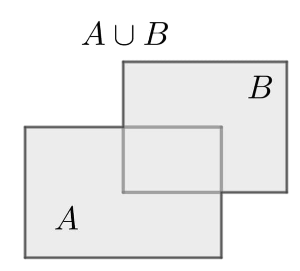
\includegraphics{cup}
\textbf{Пересечением} множеств $A$ и $B$ называется множество, состоящее из элементов принадлежащих как множеству $A$, так и множеству $B$. Обозначается как $A \cap B$.
\\ 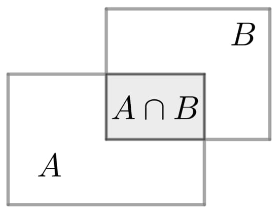
\includegraphics{dasuka}
\textbf{Разностью} множесвом $A$ и $B$ называется множество, состоящее из элементов принадлежащих множеству $A$, но не принадлежащих множеству $B$. Обозначается как $A \setminus B$.
\\ 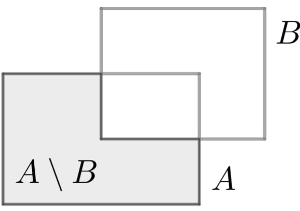
\includegraphics{vichet}
\\И о самом сложном: пусть $A$ и $B$ - множества. Тогда множество $A \times B =^{def} \{ (a, b) | a \in A \wedge b \in B \}$ называется \textbf{декартовым произведением} множества $A$ и $B$ (по картинке правда яснее).
\\ 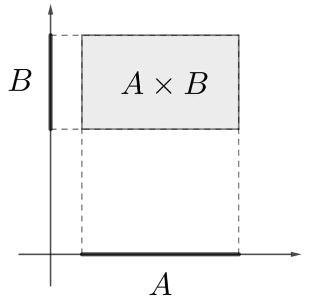
\includegraphics{decart}
Соотвественно, все приведенные выше картинки и есть \textsl{геометрические} смыслы данных операций над множествами; если у вас появились внезапные ассоциации с 9-11 классом и кругами Эйлера - не беспокойтесь, они полностью оправданы, вставьте вместо квадратов круги и грубо говоря будете правы.


\section{Отображение множества $X$ во множество $Y$. Образ и прообраз. Инъективное, сюръективное и биективное отображения. Примеры. Обратное отображение, критерий существования обратного отображения}
\textsl{Презентация по теме: 10.09.24, гл. 1, пар. 4}
\\ \\
\textbf{Отображением} $f$ множества $X$ во множество $Y$ называется правило, сопоставляющее каждому элементу $x \in X$ единственный элемент $y \in Y$. Факт отображения $f$ записывается как $f : X \to Y$ или $X \rightarrow^{f} Y$, а факт \textsl{сопоставления} элемента $x$ элементу $y$ записывается в виде $y = f(x)$ или же $x \to^{f} y$. Внимательные могли заметить что выбор буквы для обозначения отображения и сама формулировка кажется больно знакмой - оно и верно, ибо если $Y = \mathbb{R}$, то $f$ называется \textsl{функцией}.
\\ Пусть $f : X \to Y$ и $E \subset X$. Тогда множество $f(E) =^{def} \{ f(x) | x \in E \}$ называется \textbf{образом} множества $E$ при отображении $f$.
\\ 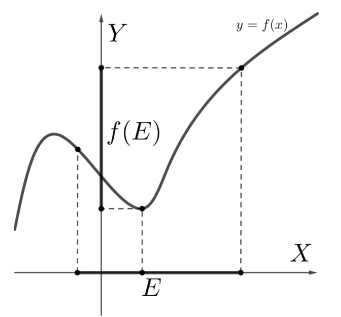
\includegraphics{obraz}
\\ И соотвественно, пусть $f : X \to Y$ и $F \subset Y$. Тогда множество $f^{-1}(F) =^{def} \{ x \in X | f(x) \in F\}$ называется \textbf{прообразом} множества $F$ при отображении $f$.
\\ 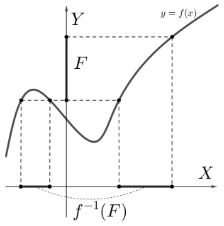
\includegraphics{proobraz}
\\В общем и целом, по-простому, по-людски, так сказать, образ - это множество значений функции от $x$ на некотором участке $E$. Прообраз - обратное действие, дающее значение всех $y$ в неком подмножестве $F$. Геометрические значения даны выше.
\\Отображением $f : X \to Y$ называется \textbf{инъекцией}, если для любых двух различных $x_{1} \in X$ и $x_{2} \in X$ верно то, что $f(x_{1}) \neq f(x_{2})$;  ну или же по более умному: $(\forall (x_{1} \in X \wedge x_{2} \in X) : x_{1} \neq x_{2}) \Rightarrow f(x_{1}) \neq f(x_{2})$
\\Отображение $f : X \to Y$ называется \textbf{сюрьекцией}, если для любого $y \in Y$ найдется $x \in X$ такой, что $f(x) = y$; иначе же - $\forall y \in Y \exists x \in X : f(x) = y$
\\По-простому же - иньекция - это ситуация, при котором для любого $x$ существует собственный \textsl{уникальный} $y$, в то время как сюрьекция - это про то, что для любого $x$ этот самый $y$ \textsl{в целом существует}. В тех случаях же, когда при отображении $f : X \to Y$ выполняются оба правила - такое отображение будет называться \textbf{биекцией}
\\В качестве примера можно просто и незамысловато привести квадратичную функцию $f(x) = x^{2}$ и рассмотреть ее при разных на разных областях определения и значения: так, например, при $X = \mathbb{R}, Y = \mathbb{R}$ не происходит ни сюрьекции, ни иньекции, зато при $X = \mathbb{R}_{+}, Y = \mathbb{R}$ происходит сюрьекция, а при $X = \mathbb{R}_{+}, Y = \mathbb{R}_{+}$ происходит биэкция. Самое сложное во всем этом не путаться между определениями, но с картинками все намного проще\dots
\\Не уверена, будет ли определение композиции отображения, потому на всякий случай замечание - \textbf{композиция отображения} это отображение сложной функции, которое обозначается как $f \circ g(x) =^{def} f(g(x))$. То бишь, $x \rightarrow^{g} y \rightarrow^{f} Z$
\\Пусть $f : X \rightarrow Y$. Отображение $g : Y \rightarrow X$ называется \textbf{обратным отображением} к $f$, если $g(f(x)) = x, \forall x \in X$ и $f(g(x)) = y, \forall y \in Y$. Обратное отображение $g$ обозначается $f^{-1}$ (то есть $f^{-1} = g$). Да, это обратная операция к отображению. Да, как $x \rightarrow^{f} y$, но $y \rightarrow^{f^{-1}} x$. 
\\\textbf{Критерий существования обратного отображения} до ужасного прост - отображение $f : X \rightarrow Y$ должно быть \textsl{биэктивно}. (теорема 4.1)

\section{Конечные, бесконечные, счетные, не более чем счетные и несчетные множества. Примеры}
\textsl{Презентация по теме: 10.09.24, 12.09.24, гл. 1, пар. 5}
\\ \\Пусть $m \in \mathbb{N}$. Множество $A$ состоит из $m$ элементов, если существует биэкция между множеством $A$ и множеством $\mathbb{N}_{m}$. Иными слвоами, элементы этого множества можно просто пронумеровать, тип раз элемент, два элемент.. пресловутый элемент номер $m$ - мы просто определяем, что воообще значит множество состоит из стольких-то элементов.
\\Множество называется \textbf{конечным}, если оно пустое или состоит из $m$ элементов для некоторого натурального $m$. Множество называется \textbf{бесконечным}, если оно не является конечным. (тупо конечное если оно имеет конец и бесконечное, если нет лмао) 
\\А теперь кайнда конфьюзинг моментс - множество $A$ называется \textbf{счетным}, если существует \textsl{биэкция} между данным множеством и множеством $\mathbb{N}$. Их можно посчитать, но вопрос \textsl{конечности} - вопрос исключительно отдельный. Если оно конечно или \textsl{бесконечно, но все элементам можно присвоить свой номер}, мы называем такое множество \textsl{не более чем счетным}, в противном случае оно \textsl{несчетное}. 
\\Немножка логичных следствий:
\begin{enumerate}
    \item Подмножество счетного множества не более чем счетно
    \item Образ счетного множества не более чем счетен
    \item Обьединение двух счетных множеств счетно
    \item Декартово произведение двух счетных множеств счетно
    \item Обьединение счетного числа счетных множеств счетно 
\end{enumerate}
Так получилось, что тут про континуальность мы не говорим. А жаль.

\section{Вещественные числа, их свойства. Верхняя и нижняя грани числовых множеств. Точные грани. Примеры. Модуль вещественного числа, его свойства.}
\textsl{Презентация по теме: 12.09.24, 17.09.24, гл. 1, пар. 6, 7}
\subsection{Вещественные числа}
Множества вещественных чисел обозначается $\mathbb{R}$. А их свойства:
\begin{enumerate}
    \item $a + b = b + a$
    \item $(a + b) + c = a + (b + c)$
    \item $a + 0 = a$
    \item $a + (-a) = 0$
    \item $a * b = b * a$
    \item $(a * b) * c = a * (b * c)$
    \item $a * 1 = a$
    \item $a * a^{-1} = 1$
    \item $(a + b) * c = a * c + b * c$
    \item если $a < b, b < c$, то $a < c$
    \item если $a < b$, то $a + c < b + c$
    \item если $a < b, c > 0$, то $a * c < b * c$
    \item если числовое множество $A$ расположено левее числового множества $B$, то найдется число $c$, лежащее между ними (свойство непрерывности). ну или же: $$((\forall A \neq \emptyset \land \forall B \neq \emptyset) : (\forall a \in A \land \forall b \in B \Rightarrow a \leq b))$$
    $$\Rightarrow (\exists c \in \mathbb{R} : (\forall a \in A \land \forall b \in B \Rightarrow a \leq c \leq b))$$
\end{enumerate}
$(\forall a \in R \land b \in \mathbb{R} : a < b) \Rightarrow (\exists r \in \mathbb{Q} : a < r < b)$, иными словами, в любом не пустом интервале найдется рациональное число).
\\Определение \textbf{модуля числа}: $$|x| =
\begin{cases}
    x, x \gg 0
\end{cases}$$
$$- x, x < 0$$
\\Не уверена, будет ли это в вопросе, но \textsl{неравенство треугольница}:
$$|a + b| \leq |a| + |b|$$
\\И \textsl{обрвтное неравенство треугольника}
$$||a| - |b|| \leq |a - b|$$
\\$\overline{\mathbb{R}} = \{-\infty \} \cup \mathbb{R} \cup \{+ \infty\}$ - \textsl{расширенная вещественная прямая}
\subsection{Точные грани числовых множеств}
Очарование данной темы в том, что оно наполнено рядами \textsl{пар} определений - аналогичные определения для чего-то большого и чего-то малого. Ситуативно начало у одного из них может как опускаться, так и нет - но суть остается той же и, вероятнее всего, каждое второе определение составлено по подобию каждого первого.
\\ Пусть $A \subset \mathbb{R}, m \in \mathbb{R}$. Если при любом $a \in A$ выполняется неравенство $a \leq m$, то число $m$ называетя \textbf{верхнью гранью множества} $A$. Если же $k \in \mathbb{R}$ и $a \geq k$, то $k$ называется \textbf{нижнью гранью числвого множества} $A$. Данные грани определны неоднозначно и любое число выходящее за них (больше верхнего или меньше нижней) является данной гранью.
\\ Числовое множество называется \textbf{ограниченным сверху}, если у этого множества существует верхняя грань. Числовое множество называется \textbf{ограниченным снизу}, если у этого множества есть нижняя грань. Числовое множество называется \textbf{ограниченным}, если оно ограничено и сверху, и снизу. Оно так же может быть неограниченным, да, та же логика (из примеров $\mathbb{N, Q, R}$)
\\Пусть $A \subset \mathbb{R}$. Если $q \in A$ и при любом $a \in A$ выполняется неравенство $a \leq p$, то число $p$ называется \textbf{максимальным (наибольшим) элементом} множества $A$. Максимальный элемент обозначается \textsl{max $A$}. Если при тех же вводных выполняется неравенство $a \geq q$, то число $q$ называется \textbf{минимальным (наименьшим) элементом} множества $A$. Минимальный элемент обозначается \textsl{min $A$}. Данные элементы не всегда существуют, например если $A = [0, 1)$ наименьший элемент будет равен 0, а наибольшего не сущесвтует.
\\Пусть $A \subset \mathbb{R}$ - непустое. Если $A$ ограничено сверху, то его \textsl{точной верхней гранью} (лат. supremum - наибольший) будем называть н\textsl{аименьшую из верхних граней множества} $A$. Если $A$ неограничено сверху, то его точной верхней гранью будем считать $+\infty$. Точная верхняя грань обозначается \textsl{sup $A$}. И, опять-таки, при тех же началах, если $A$ ограничено снизу, то его т\textsl{очной нижней гранью} (лат. infinum - наименьший) будем называть \textsl{наибольшую из нижних граней множества} $A$, если оно неограничено, нижняя грань - $-\infty$, точная грань обозначается \textsl{inf $A$}. Типа, $sup[0, 1) = 1, inf[0, 1) = 0$. 
\\\textbf{У любого непустого числового множества существует точные верхняя и нижняя грани.}


\section{Лемма о вложенных сегментах.}
\textsl{Презентация по теме: 17.09.24, гл. 1, пар. 7}
\\ \\ \textbf{Лемма о вложенных сегментах:} пусть $[a_{n}, b_{n}], n \in \mathbb{N}$ замкнутные промежутки такие, что
\begin{enumerate}
    \item $[a_{n}, b_{n}] \supset [a_{n+1}, b_{n+1}]$ при всех $n \geq 1$
\\ \\Тогда $\exists c \in \mathbb{R}$ такое, что при всех $n \geq 1$ выполнено $c \in [a_{n}, b_{n}]$. Если дополнительно предположить, что 
    \item $inf {b_{n} - a_{n}|n \in \mathbb{N}} = 0$
\\ \\то такое число $c$ единственно.
\end{enumerate}
Теперь страшное. \textbf{Доказательство:}
\\ 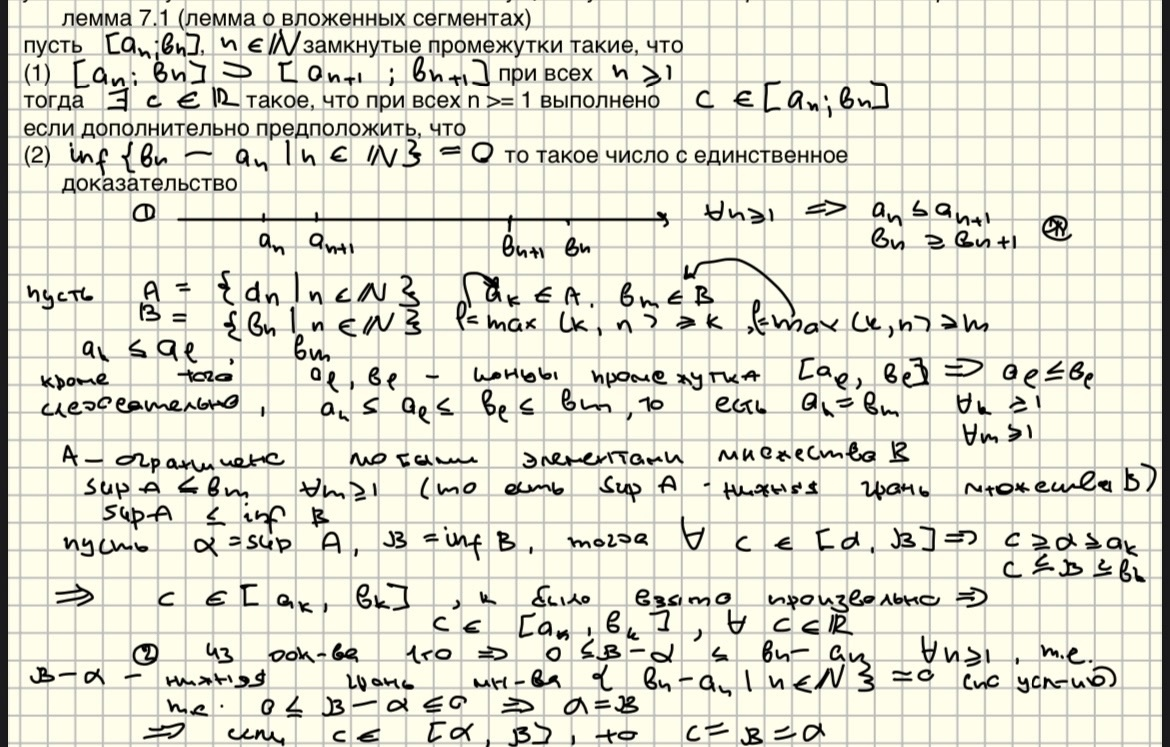
\includegraphics[width=1\linewidth]{lemmasegm}

\section{Окрестности. $\varepsilon $-окрестности, их геометрический смысл, запись в виде неравенства. Свойства окрестностей.}
\textsl{Презентация по теме: 17.09.24, 19.09.24, гл. 1, пар. 8}
\\ \\Точно так же, как и с точными гранями множеств, тут будут ряды однотипных определений, только в несколько раз хуже - это будут не пары, а натурально \textsl{ряды} для разных случаев под разные возможности. Опять-таки, порой начало будет опускаться и из-за этого будет казаться более сжатым или непонятным. Просто держите в голове это.
\\Пусть $a \in \mathbb{R}$. Интервал, содержащий точку $a$, называется \textbf{окрестностью $a$}. Окрестности обозначаются $U(a), V(a), W(a)$
\\Пусть теперь $\lambda \in \mathbb{R}$. Интервал $(\lambda, + \infty)$ называется \textsl{окрестностью $+ \infty$}. Аналогично интервал $(-\infty, \mu )$ при $\mu \in \mathbb{R}$ называется \textsl{окрестностью $-\infty$}. Если же интервал $(-\infty, \mu) \cup (\lambda, +\infty)$ - он называется \textsl{окрестностью $\infty$}.
\subsection{Окрестности для разных интервалов}
\begin{enumerate}
    \item Пусть $a \in \mathbb{R}, \varepsilon > 0$. Интервал $(a - \varepsilon, a + \varepsilon)$ называется $\varepsilon$ - окрестностью $a$. $$x \in U_{\varepsilon}(a) \Leftrightarrow |x - a| < \varepsilon $$ $$x \in \stackrel{\circ}{U}_{\varepsilon}(a) \Leftrightarrow 0 < |x - a| < \varepsilon$$
    \item Пусть $\varepsilon > 0$. Интервал $(\varepsilon, +\infty)$ называется $\varepsilon$ - окрестностью $+\infty$. $$x \in U_{\varepsilon}(+\infty) \Leftrightarrow x > \varepsilon$$
    \item Пусть $\varepsilon > 0$. Интервал $(-\infty, -\varepsilon)$ называется $\varepsilon > 0$ - окрестностью $-\infty$. $$x \in U_{\varepsilon}(-\infty) \Leftrightarrow x < -\varepsilon$$
    \item Пусть $\varepsilon > 0$. Интервал $(-\infty, -\varepsilon) \cup (\varepsilon, +\infty)$ называется $\varepsilon$ - окрестностью $\infty$. $$x \in U_{\varepsilon}(\infty) \Leftrightarrow |x| > \varepsilon$$
\end{enumerate}
Небольшая перебивочка на обьяснение некоторых обозначений. Пусть $A \subset \mathbb{R}, B \subset \mathbb{R}, \alpha \in \mathbb{R}$, тогда
\begin{enumerate}
    \item $\alpha * A \stackrel{def}{=} \{\alpha * a | a \in A\}$
    \item $A + B \stackrel{def}{=} \{a + b | a \in A, b \in B\}$
    \item $A * B \stackrel{def}{=} \{a * b | a \in A, b \in B\}$
    \item $A^{-1} \stackrel{def}{=} \{ \frac{1}{a} | a \neq 0, a \in A\}$
\end{enumerate}
\subsection{Свойства окрестностей}
\begin{enumerate}
    \item Пусть $a \in \overline{\mathbb{R}}$. Тогда для любой окрестности U(a) точки a найдется $\varepsilon > 0$ такое, что $V_{\varepsilon} \subset U(a)$
    \item Если $a, b \in \overline{\mathbb{R}}$ и $a \neq b$, то существуют окрестности U(a) и V(b) такие что $U(a) \cap V(b) =  \emptyset$
    \item Если U(a) и V(b) - окрестности точки a, то $U(a) \cap V(a)$ - окрестности точки a
    \item Если $p, q \in U(a)$, то $[p, q] \subset U(a)$
    \item Пусть $a, b, c \in \mathbb{R}$ и $a = b + c$. Тогда для любой окрестности U(a) найдутся окрестности V(b) и W(c) такие, что $V(b) + W(c) \subset U(a)$
    \item Пусть $a, b, c \in \mathbb{R}$ и $a = b * c$. Тогда для любой окрестности U(a) найдутся окрестности V(b) и W(c) такие, что $V(b) * W(c) \subset U(a)$
    \item Пусть $a \in \mathbb{R}$ и $a \neq 0$. Тогда для любой окрестности $U(\frac{1}{a})$ найдется окрестности V(a) такая, что $(V(a))^{-1} \subset U(\frac{1}{a})$
\end{enumerate}
Там включены доказательства, но опять-таки ни слова о том, что это будет спрашиваться - но, де-юре, упражнения на раскрытие определения окрестностей и последующую арифметику.

\section{Понятие последовательности, монотонные последовательности. Ограниченные и неограниченные последовательности. Примеры}
\textsl{Презентация по теме:19.09.24, гл. 2, пар. 1}
\\ \\Отображение $x : \mathbb{N} \rightarrow \mathbb{R}$ из множества натуральных чисел называется \textbf{числовой последовательностью}. $x_{n} \stackrel{def}{=} x(n)$ называют n-ым (или общим) членом последовательности, а саму последовательность обозначают как\textsl{ $\{x_{n}\}^{\infty}_{n = 1}$}. n - натуральное число, переменная, принимающие сколь угодно большие значения, но не меньшая чем 1.
\\Пусть $\{x_{n}\}^{\infty}_{n = 1}$ - числовая последовательность, $m \in \mathbb{N}$. Обозначим за $y_n = x_{n + m}$. Тогда последовательность $\{y_{n}\}^{\infty}_{n = 1}$ называется (m-ым) \textbf{остатком последовательности} $\{x_{n}\}^{\infty}_{n = 1}$. Или же - остаток - это те члены последовательности, которые остались после отбрасывания первых m членов.
\\А теперь, \textbf{определения ограниченностей}, господи боже:
\begin{itemize}
    \item Последовательность $\{x_{n}\}^{\infty}_{n = 1}$ называется \textsl{ограниченной сверху}, если найдется такое число $A$, что при
    \item Последовательность $\{x_{n}\}^{\infty}_{n = 1}$ называется \textsl{ограниченной снизу}, если найдется такое число $B$, что при любом натуральном n выполняется неравенство $x_n \geq B$
    \item Последовательность $\{x_{n}\}^{\infty}_{n = 1}$ называется \textsl{ограниченной}, если она ограничена сверху и снизу
    \item Последовательность $\{x_{n}\}^{\infty}_{n = 1}$ называется \textsl{неограниченной}, если она не является ограниченной
\end{itemize}
\textbf{\\Про возрастания-убывания-прочие:}
\begin{itemize}
    \item Последовательность $\{x_{n}\}^{\infty}_{n = 1}$ называется \textsl{возрастающей}, если $x_{n} < x_{n + 1}$ при любом натуральном n.
    \item Последовательность $\{x_{n}\}^{\infty}_{n = 1}$ называется \textsl{убывающей}, если $x_{n} > x_{n + 1}$ при любом натуральном n.
    \item Последовательность $\{x_{n}\}^{\infty}_{n = 1}$ называется \textsl{неубывающей}, если $x_{n} \leq x_{n + 1}$ при любом натуральном n.
    \item Последовательность $\{x_{n}\}^{\infty}_{n = 1}$ называется \textsl{невозрастающей}, если $x_{n} \geq x_{n + 1}$ при любом натуральном n.
\end{itemize}
Последовательность называется \textbf{монотонной}, если она что угодно из тех четырех определений вверху; последовательность называется \textbf{строго монотонной} только если она либо возрастающая, либо убывающая.
\\Пусть $\{x_{n}\}^{\infty}_{n = 1}$ - числовая последовательность, а $\{n_{k}\}^{\infty}_{k = 1}$ - возрастающая последовательность натуральных чисел. Обозначим $y_{k} = x_{nk}$. Тогда последовательность $\{y_{k}\}^{\infty}_{k = 1}$ называется \textbf{подпоследовательностю} $\{x_{n}\}^{\infty}_{n = 1}$. подпоследовательность получается из исходной последовательности вычеркиванием каких-либо из членов последовательности, да, сюда входят остатки последовательносей.

\section{Определение предела последовательности, геометрический смысл. Сходящиеся и расходящиеся последовательности. Примеры.}
\textsl{Презентация по теме: 19.09.24, 26.09.24, гл. 2, пар. 2}
\\ \\ Пусть $\{x_{n}\}^{\infty}_{n = 1}$ - числовая последовательность $a \in \bar{\mathbb{R}} \cup \{\infty\}$. a называют \textbf{пределом последовательности} $\{x_{n}\}^{\infty}_{n = 1}$ при стремлении n к $+ \infty$ и обозначают $\lim_{n \to \infty} x_{n} = a$, если 
$$\forall U(a) \exists N_{\varepsilon} \in N : (\forall n > N \Rightarrow x_{n} \in U(a))$$
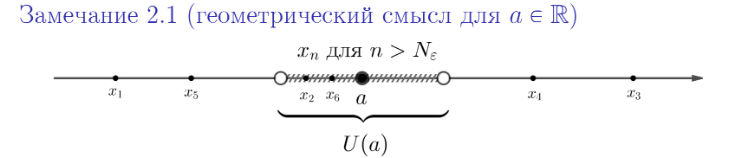
\includegraphics[width=1\linewidth]{predelposl}
\\ Для любой окрестности U(a) найдется номер N (зависящий от U(a)) после которого члены последовательности попадают внутрь этой окрестности. 
\\ $a = \lim_{n \to \infty} x_n \Leftrightarrow$ В любой окрестености точки a содержаться все члены последовательности за исключением конечного числа.
\subsection{Частные случаи определения предела последовательности}
\begin{itemize}
    \item Пусть $\{x_{n}\}^{\infty}_{n = 1}$ - числовая последовательность $a \in \mathbb{R}$. a называют пределом последовательности $\{x_{n}\}^{\infty}_{n = 1}$ при стремлении n к $+ \infty$ и обозначают $\lim_{n \to \infty} x_{n} = a$, если $$\forall \varepsilon > 0 \exists N_{\varepsilon} : (\forall n > N_{\varepsilon} \Rightarrow |x_n - a| < \varepsilon)$$
    \item Пусть $\{x_{n}\}^{\infty}_{n = 1}$ - числовая последовательность. $+ \infty$ называют пределом последовательности $\{x_{n}\}^{\infty}_{n = 1}$ при стремлении n к $+ \infty$ и обозначают $\lim_{n \to \infty} x_{n} = +\infty$, если $$\forall \varepsilon > 0 \exists N_{\varepsilon} : (\forall n > N_{\varepsilon} \Rightarrow x_n < \varepsilon)$$
    \item Пусть $\{x_{n}\}^{\infty}_{n = 1}$ - числовая последовательность. $- \infty$ называют пределом последовательности $\{x_{n}\}^{\infty}_{n = 1}$ при стремлении n к $+ \infty$ и обозначают $\lim_{n \to \infty} x_{n} = -\infty$, если $$\forall \varepsilon > 0 \exists N_{\varepsilon} : (\forall n > N_{\varepsilon} \Rightarrow x_n < - \varepsilon)$$
    \item Пусть $\{x_{n}\}^{\infty}_{n = 1}$ - числовая последовательность. $\infty$ называют пределом последовательности $\{x_{n}\}^{\infty}_{n = 1}$ при стремлении n к $+ \infty$ и обозначают $\lim_{n \to \infty} x_{n} = \infty$, если $$\forall \varepsilon > 0 \exists N_{\varepsilon} : (\forall n > N_{\varepsilon} \Rightarrow |x_n| < \varepsilon)$$
\end{itemize}
И только заметила, но удивительно нигде не дано обьяснение тому, что такое \textsl{сходящееся последовательность}. Так вот, это та последовательность, у которой есть предел. 
\\ Пусть $\{x_{n}\}^{\infty}_{n = 1}$ и $\{y_{n}\}^{\infty}_{n = 1}$ - \textsl{сходящиеся} последовательности. Тогда
\begin{enumerate}
    \item Если $\alpha \in \mathbb{R}$, то $\lim_{n \to \infty}(\alpha * x_n) = \alpha * \lim_{n \to \infty}(x_n)$
    \item $\lim_{n \to \infty}(x_n + y_n) = \lim_{n \to \infty}(x_n) + \lim_{n \to \infty}(y_n)$  
    \item $\lim_{n \to \infty}(x_n * y_n) = \lim_{n \to \infty}(x_n) * \lim_{n \to \infty}(y_n)$ 
    \item Если $\lim_{n \to \infty}(y_n) \neq 0$, то $\lim_{n \to \infty}\frac{x_n}{y_n} = \frac{\lim_{n \to \infty}(x_n)}{\lim_{n \to \infty}(y_n)}$
\end{enumerate}

\end{document}
